\documentclass[10pt, pdf, xcolor=pdftex, dvipsnames, table]{beamer}

%\usepackage[brazil]{babel}
\usepackage[english]{babel}
\usepackage[utf8]{inputenc}
\usepackage[T1]{fontenc}
\usepackage{amsfonts}
\usepackage{amsmath}
\usepackage{algorithm}
\usepackage{algpseudocode}
\usepackage{pgfpages}
\usepackage{fancyvrb}
\usepackage{times}
\usepackage{amsmath,amssymb}
\usepackage{graphicx}
\usepackage{hyperref}
\usepackage{pxfonts,txfonts}
\usepackage{url}
\usefonttheme{structurebold}
\usepackage{hyphenat}
\usepackage{multicol}
\usepackage{palatino}
\usepackage[normalem]{ulem}
\usepackage{booktabs}
\useunder{\uline}{\ul}{}
\usepackage{appendix}
\usepackage{float}
\usepackage{verbatim}
\usepackage{cooltooltips}
\usepackage{paralist}
\usepackage[inline]{enumitem}
\usepackage{multirow}
\usepackage{array}
\usepackage{xargs}
\usepackage{xcolor}
\usepackage{subfigure}
\usepackage{caption}
%\usepackage{bm}

\captionsetup{font=scriptsize,labelfont=scriptsize}
\captionsetup{skip=1pt,belowskip=1pt}

\definecolor{mygray}{gray}{0.8}

\newtheorem{hipotese}{Hipótese}

\usepackage{listings} % para inserir codigo fonte
\lstset{extendedchars=true,frame=tb,basicstyle=\footnotesize,stringstyle=\ttfamily,showstringspaces=true}

\renewcommand{\lstlistingname}{Listagem}

\newcommand{\x}{\textbf{\textcolor{Green}{$\surd$}}}
\newcommand{\xx}{\textbf{\textcolor{Blue}{$\odot$}}}
\newcommand{\xxx}{\textbf{\textcolor{Red}{$\times$}}}

\usetheme{Amsterdam}
\usefonttheme[onlymath]{serif}

\floatname{algorithm}{Algoritmo}

%\newenvironment<>{varblock}[2][.9\textwidth]{%
%\setlength{\textwidth}{#1}
%	\begin{actionenv}#3%
%    		\def\insertblocktitle{#2}%
%    		\par%
%    		\usebeamertemplate{block begin}}
%  		{\par%
%    		\usebeamertemplate{block end}%
%  	\end{actionenv}}

% Efeitos:
\transdissolve %dissolve a lamina anterior;
% \transsplitverticalout % a proxima lamina se abre como uma cortina no sentido horizontal;
% \transblindshorizontal % a lamina anterior converte-se linha a linha.

% Para gerar apenas as páginas sem efeitos de overlay use (bom para imprimir):
% \usepackage[handout]{beamer}

% Para colocar número de páginas no slide:
%\setbeamertemplate{footline}[frame number]

% Para retirar a barra de navegação:
\setbeamertemplate{navigation symbols}{}

% Ativa ou desativa as anotações
\setbeameroption{hide notes}
%\setbeameroption{show notes}

% Ativa númeração de figuras
\setbeamertemplate{caption}[numbered]

% inserir logotipo a apresentação
\pgfdeclareimage[height=1.5cm]{logo}{images/lups_oficial.png}
\logo{\pgfuseimage{logo}}

%==================================================================================

%EVENTO
%\renewcommand{\evento}{Apresentação de artigo - Metodologia para pesquisa e desenvolvimento em Computação }

% TITULO DA APRESENTACAO
\title{Mobility-Aware Application Scheduling in Fog Computing}

%Autor
\author{Luiz F. Bittencourt %$^{1}$
\and Javier Diaz-Montes %$^{1}$
\and Rajkumar Buyya %$^{2}$
\and Omer F. Rana
\and Manish Parashar
\newline
\newline
\and Presenter: Maicon Ança dos Santos
}

%%%%%%%%%%%%%%%%%%%%%%%%%%%%%%%%%%%%%%%%
% Instituição , 
%%%%%%%%%%%%%%%%%%%%%%%%%%%%%%%%%%%%%%%%

%\institute{1\quad Department of Computer Engineering, University of Science and Culture, Tehran, Iran \\ 2\quad School of Computer Engineering, Iran University of Science and Technology, Tehran, Iran
%}

%\date{\today}

\begin{document}

\frame{\titlepage}
\pgfdeclareimage[height=0.7cm]{logo}{images/lups_timbre.png}
\logo{\pgfuseimage{logo}}
%\frame{\tableofcontents}


%%%%%%%%%%%%%%%%%%%%%%%%%%%%%%%%%%%%%%%%%%%%%
% Conteúdo da Apresentação
%%%%%%%%%%%%%%%%%%%%%%%%%%%%%%%%%%%%%%%%%%%%%

\section[Introduction]{Introduction}

%\begin{frame}
%	\tableofcontents[currentsection]
%\end{frame}

\begin{frame}
	\frametitle{Introduction}
 	\begin{block}{}
 		\begin{itemize}
 			\item[•] With new levels of computing capacity provides by Fog computing, new forms of resource allocation and management can be developed;
 		    	\item[•] The grow of the number of devices scattered and connected to Internet, producing and consuming data, requires a scalable resource management at unprecedented levels
 		    	\begin{itemize}
 		    		\item[-] \footnotesize\textit{Focus on IoT}
			\end{itemize}
 		\end{itemize}
 	\end{block}
\end{frame}

\begin{frame}
	\frametitle{Introduction}
 	\begin{block}{}
 		\begin{itemize}
 			\item[•] Data also are produced at the edge. Data generation and consumption can occur at many differents places and times;
 			\newline
 		    \item[•] Different applications can have different requirements, especially in terms of response time.
 		\end{itemize}
 	\end{block}
\end{frame}

\begin{frame}
	\frametitle{Introduction}
 	\begin{block}{The problem}
 			\textit{\newline \textbf{Resource allocation considering the hierarchical infrastructure composed of edge capacity and cloud data centers, analyzing application classes along with different scheduling policies.}\newline}
 	\end{block}
\end{frame}

\section[Fog Computing Model]{Fog Computing Model}

\begin{frame}
	\tableofcontents[currentsection]
\end{frame}

\begin{frame}
	\frametitle{Fog Computing Model}
 	\begin{block}{}
 		\begin{itemize}
 		    \item[•] User applications that access the public cloud do so through an access point that allows data exchange through the core network to reach the cloud data center;\newline
 		    \item[•] \emph{Cloudlet}: access point extended to also provide computing and storage services.
 		\end{itemize}
 	\end{block}
\end{frame}

\begin{frame}
 	\begin{figure}[htbp]
 		\centerline{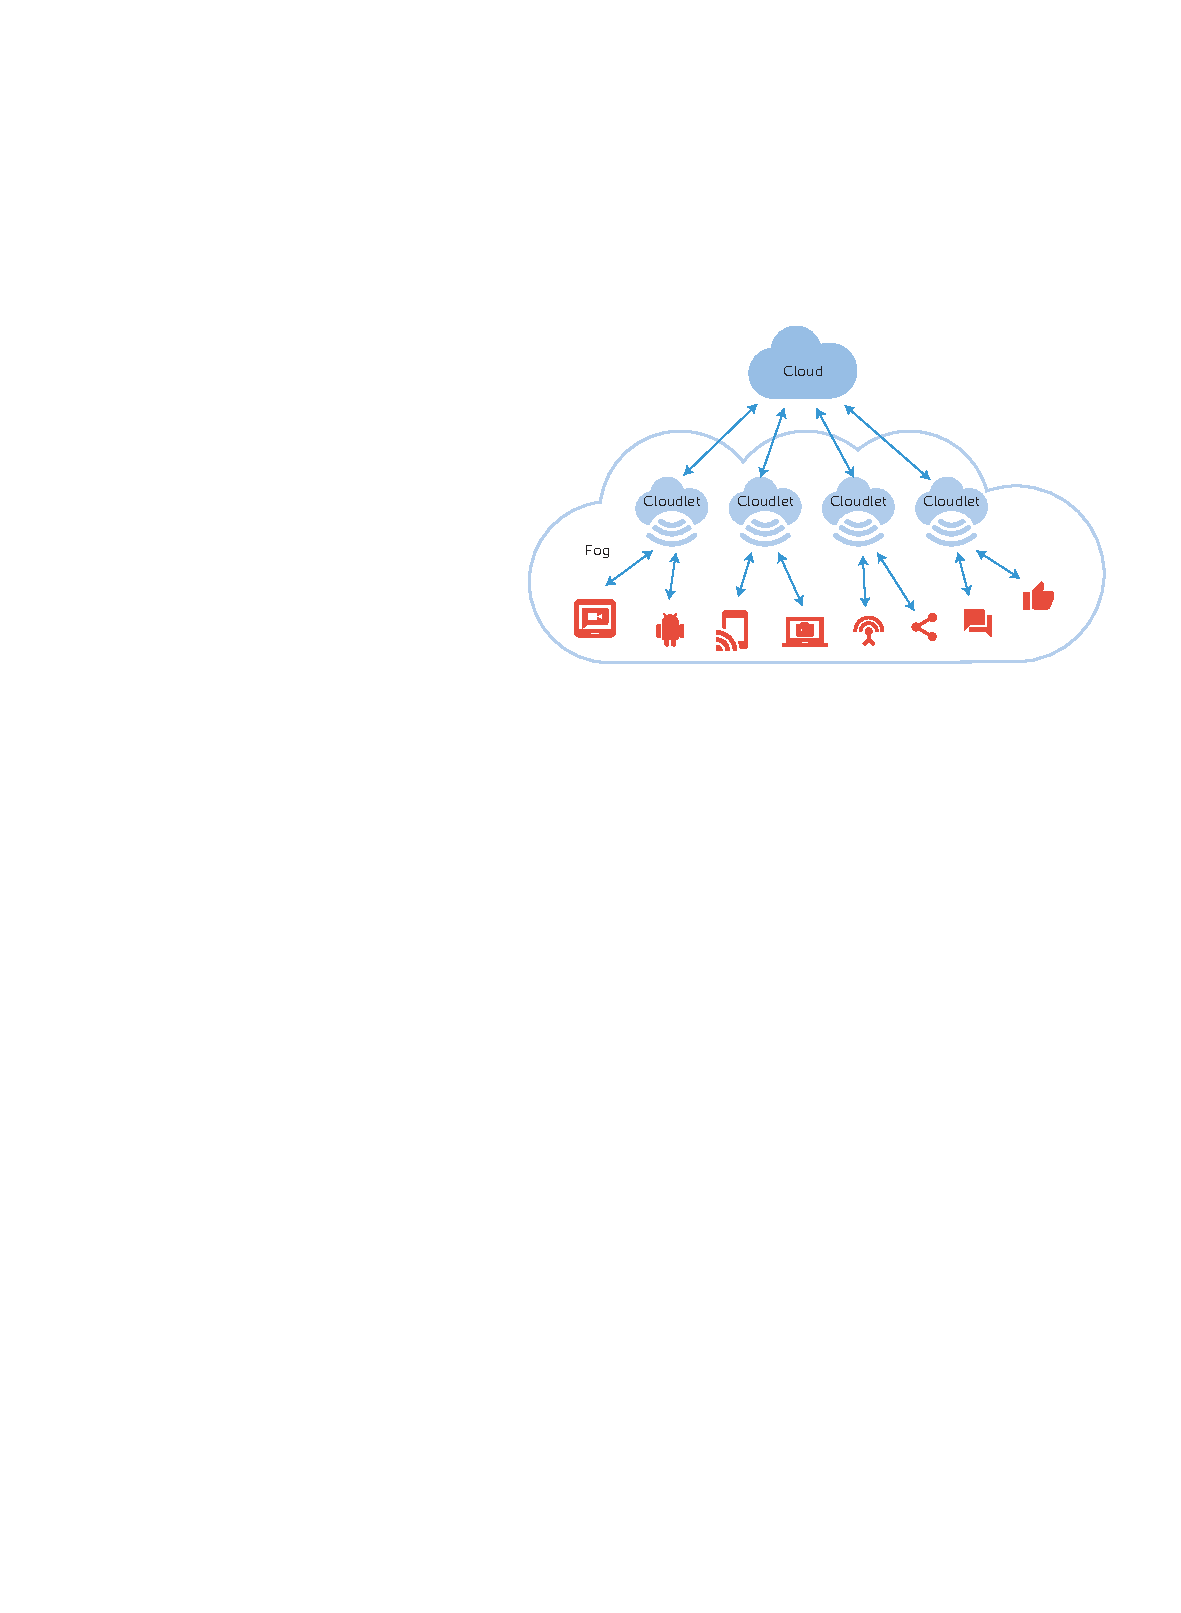
\includegraphics[scale=1]{images/fog.pdf}}
 		\caption[Fog computing: cloud, cloudlets and edge devices/applications ecosystem]{Fog computing: cloud, cloudlets and edge devices/applications ecosystem}
 	\end{figure}
\end{frame}

\begin{frame}
	\frametitle{Fog Computing Model}
 	\begin{block}{}
 		\begin{itemize}
 		     \item[•] Hierarchical, bi-directional computing infrastructure: edge devices communicate with cloudlets and cloudlets communicate with clouds.\newline
 		    	\begin{itemize}
 		    		\item[-] \footnotesize\textit{Cloudlets can also communicate with each other to perform data and process management.}
 		    	\end{itemize}
 		\end{itemize}
 	\end{block}
\end{frame}

\begin{frame}
	\frametitle{Fog Computing Model}
 	\begin{block}{}
 		\begin{itemize}
 		     \item[•] Processing and storage capacity in fog computing can benefit different types of applications\newline
 		    	\begin{itemize}
 		    		\item[-] \footnotesize\textit{Applications with low latency requirements;}\newline
 		    		\item[-] \footnotesize\textit{Applications that currently rely on the cloud;}\newline
 		    		\item[-] \footnotesize\textit{Cases in which raw data collected by many devices that generally do not need to be transferred to the cloud for long-term storage.}
 		    	\end{itemize}
 		\end{itemize}
 	\end{block}
\end{frame}

\begin{frame}
	\frametitle{Fog Computing Model}
 	\begin{block}{}
 		\begin{itemize}
 		     \item[•] Cloudlets can provide reduced latencies, however...\newline
 		    	\begin{itemize}
 		    		\item[-] \footnotesize\textit{New challenges: \textbf{what}, \textbf{when} and \textbf{where} carry out processing to meet QoS;}\newline
 		    		\item[-] \footnotesize\textit{Fog scheduling must bring users location to the resource allocation policies to uphold the benefits of proximity to the user.}
 		    	\end{itemize}
 		\end{itemize}
 	\end{block}
\end{frame}

\section[Related Work]{Related Work}

\begin{frame}
	\tableofcontents[currentsection]
\end{frame}

\begin{frame}
	\frametitle{Related Work}
 	\begin{block}{}
 		\begin{itemize}
 		    \item[•] Fog computing as a platform to provide support  for IoT;\newline
 		    \item[•] A programming model has been proposed to support fog computing applications, which includes event handlers and APIs;\newline
 		    \item[•] GigaSight is a virtual machine-based cloudlet infrastructure used to support video storage analytics at the edge.
 		\end{itemize}
 	\end{block}
\end{frame}

\begin{frame}
	\frametitle{Related Work}
 	\begin{block}{}
 		\begin{itemize}
 		    \item[•] Resource management objectives and challenges in cloud computing; resource management functions and network-aware resource allocation;\newline
 		    \item[•] Multi-clouds are platforms that aggregate computing resources from different cloud providers;\newline
 		    \item[•] The ETSI has launched the initiative to create standards for mobile edge computing platforms, having proposed a blueprint and also documents presenting technical requirements, terminology, and service scenarios.
 		\end{itemize}
 	\end{block}
\end{frame}

\section[Applications]{Applications}

\begin{frame}
	\tableofcontents[currentsection]
\end{frame}

\begin{frame}
	\frametitle{Applications}
 	\begin{block}{}
 		\begin{itemize}
 		    \item[•] The fog architecture is hierarchical, where the decision is subject to application constraints and user geo-location\newline
 				\begin{itemize}
 		    		\item[-] \footnotesize\textit{Application constraints can be specified, for instance, as in the form of QoS constraints;}\newline
 		    		\item[-] \footnotesize\textit{User geo-location depends on human behavior.}
 		    	\end{itemize}
 		\end{itemize}
 	\end{block}
 	\footnotesize\textit{\textbf{"By acknowledging different application classes, one could employ different scheduling policies, algorithms, or mechanisms to deal with each class."}}
\end{frame}

\subsection[Application Model]{Application Model}

\begin{frame}
	\frametitle{Applications}
 	\begin{block}{}
 		\begin{itemize}
 		    \item[•] Considering geo-location and different application classes, were identified two types of apps:\newline
 				\begin{itemize}
 		    		\item[-] \footnotesize\textit{Near real-time: EEGTBG game;}\newline
 		    		\item[-] \footnotesize\textit{Delay-tolerant: VSOT application.}
 		    	\end{itemize}
 		\end{itemize}
 	\end{block}
\end{frame}

\begin{frame}
 	\begin{figure}[htbp]
 		\centerline{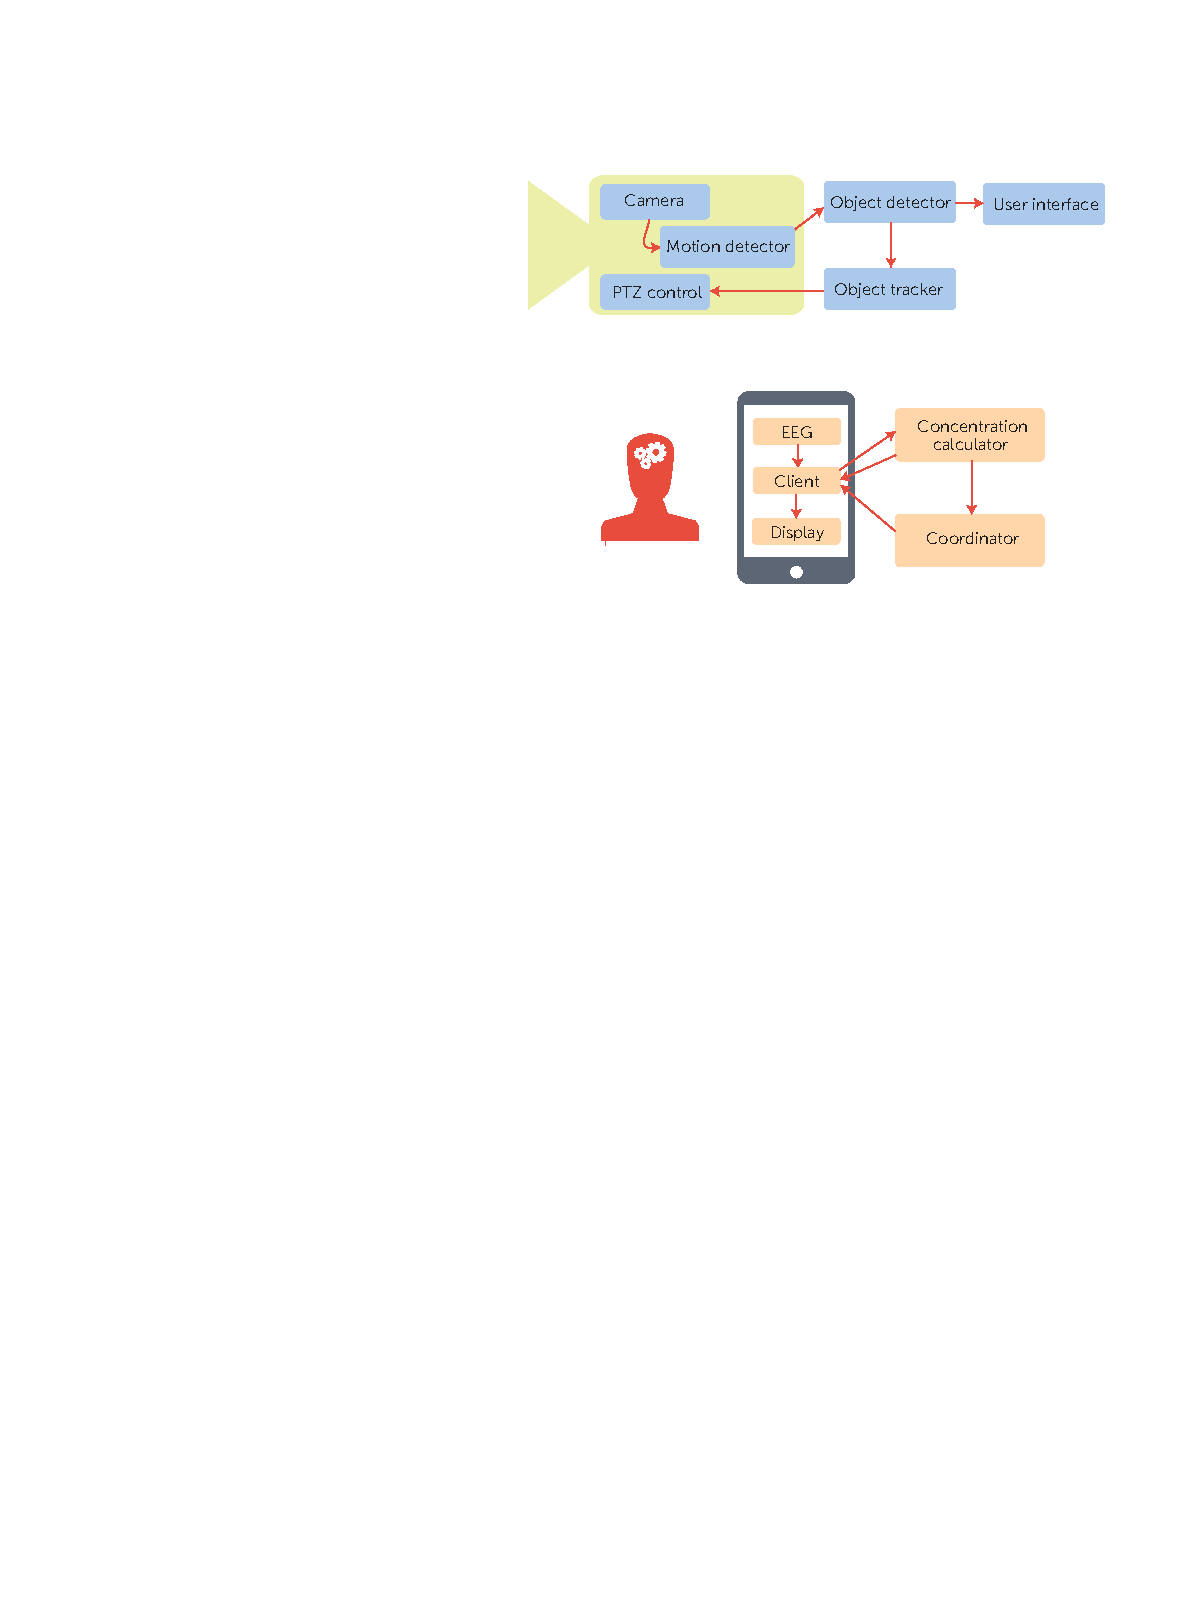
\includegraphics[scale=0.9]{images/apps.pdf}}
 		\caption[Example applications and their modules]{Example applications and their modules}
 	\end{figure}
\end{frame}

\begin{frame}
	\frametitle{Applications}
 	\begin{block}{}
 		\begin{itemize}
 		    \item[•] Electroencephalography tractor beam game (EEGTBG):\newline
 				\begin{itemize}
 		    		\item[-] \footnotesize\textit{Players try to gather items by concentrating on them. A player that has a better concentration on an item can attract it towards him/herself;}\newline
 		    		\item[-] \footnotesize\textit{Fast processing and low response times achieved by edge computing devices can give players a true online, real-time experience.}
 		    	\end{itemize}
 		\end{itemize}
 	\end{block}
\end{frame}

\begin{frame}
	\frametitle{Applications}
 	\begin{block}{}
 		\begin{itemize}
 		    \item[•] Video surveillance/object tracking application (VSOT):\newline
 				\begin{itemize}
 		    		\item[-] \footnotesize\textit{Set of distributed intelligent cameras that are able to track movement, having 6 modules: camera, motion detector, object detector, object tracker, user interface, and pan, tilt, and zoom (PTZ) control.}\newline
 		    	\end{itemize}
 		\end{itemize}
 	\end{block}
\end{frame}

\begin{frame}
	\frametitle{Applications}
 	\begin{block}{}
 		\begin{itemize}
 		    \item[•] EEGTBG (delay-sensitive) and VSOT (delay-tolerant) can be set up in a fog to take advantage of low latency due to the use of cloudlets\newline
 				\begin{itemize}
 		    		\item[-] \footnotesize\textit{VSOT is able to work under data center-distance latencies >100 miliseconds;}\newline
 		    		\item[-] \footnotesize\textit{In EEGTBG, higher delays can impact the players real-time perception, making the game unreal and impairing its playability.}
 		    	\end{itemize}
 		\end{itemize}
 	\end{block}
\end{frame}

\subsection[Mobility Scenario]{Mobility Scenario}

\begin{frame}
 	\begin{figure}[htbp]
 		\centerline{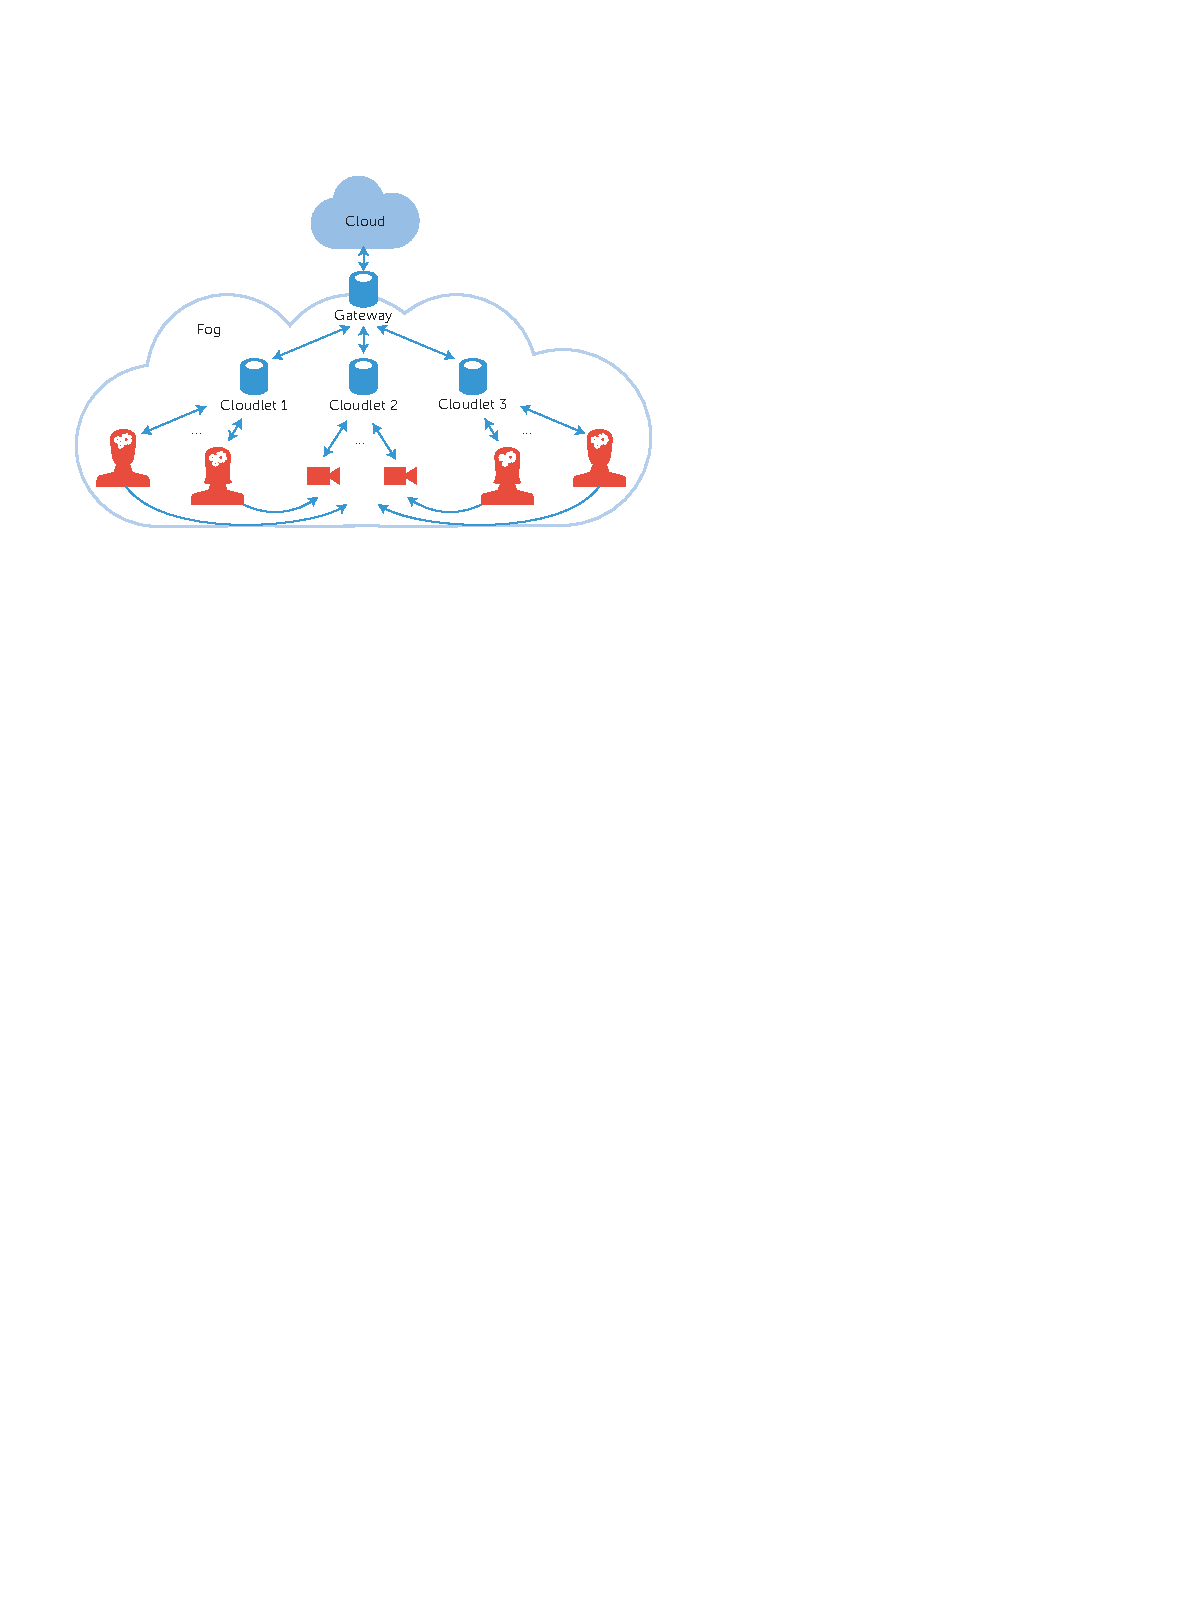
\includegraphics[scale=0.9]{images/mobility.pdf}}
 		\caption[Mobility scenario: mobile concentration game users electroencephalography tractor beam game (EEGTBG) move and compete for the same cloudlet resources with existing surveillance (VSOT) application]{Mobility scenario: mobile concentration game users electroencephalography tractor beam game (EEGTBG) move and compete for the same cloudlet resources with existing surveillance (VSOT) application}
 	\end{figure}
\end{frame}

\section[Allocation Policies]{Allocation Policies}

\begin{frame}
	\tableofcontents[currentsection]
\end{frame}

\begin{frame}
	\frametitle{Allocation Policies}
 	\begin{block}{Scheduling Strategies}
 		\begin{itemize}
 		    \item[•] \textbf{\textit{Concurrent}}: application requests that arrive at a cloudlet are simply allocated to such cloudlet, regardless of capacity or current usage;\newline
 		    \item[•] \textbf{\textit{First Come-First Served (FCFS)}}: requests are served in the order of their arrival, until there are no more computing resources available;\newline
 		    \item[•] \textbf{\textit{Delay-priority}}: applications requiring lower-delay are scheduled first.
 		\end{itemize}
 	\end{block}
\end{frame}

\subsection[Results]{Results}

\begin{frame}
 	\begin{figure}[htbp]
 		\centerline{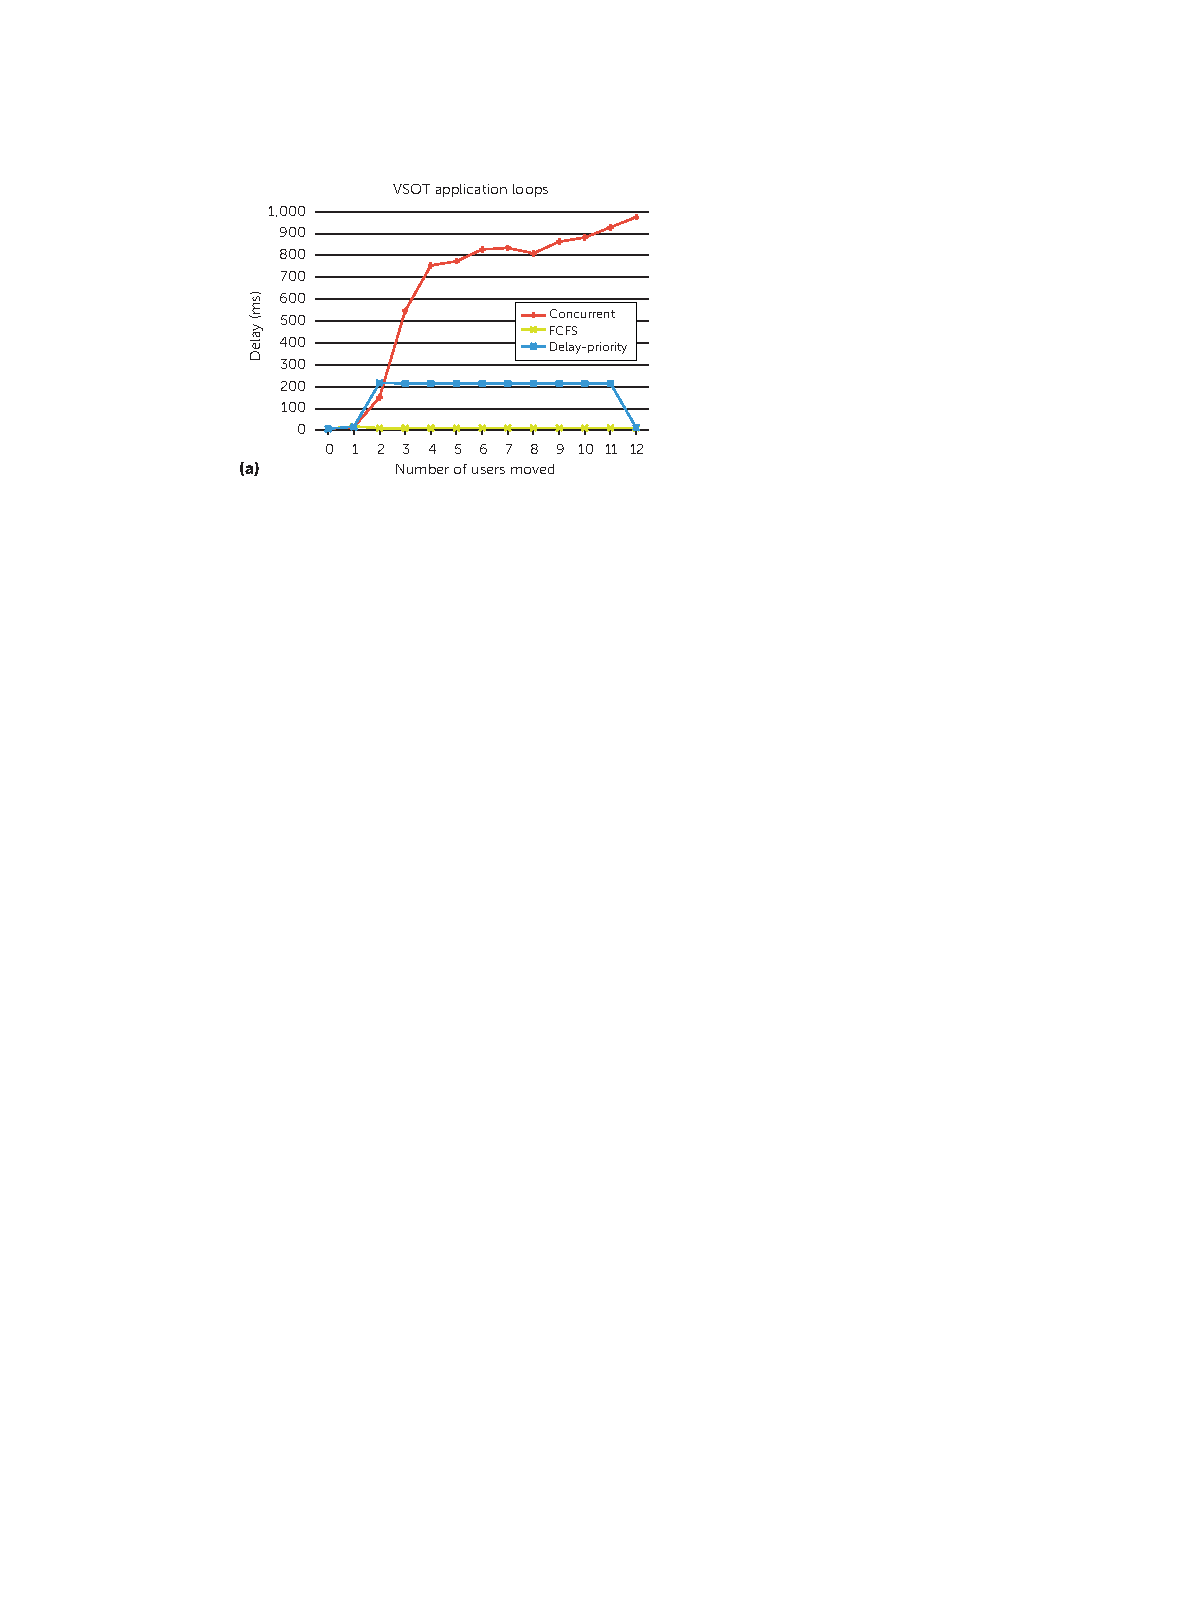
\includegraphics[scale=1.2]{images/4a.pdf}}
 		\caption[Application loop delays according to the scheduling strategy]{Application loop delays according to the scheduling strategy}
 	\end{figure}
\end{frame}

\begin{frame}
 	\begin{figure}[htbp]
 		\centerline{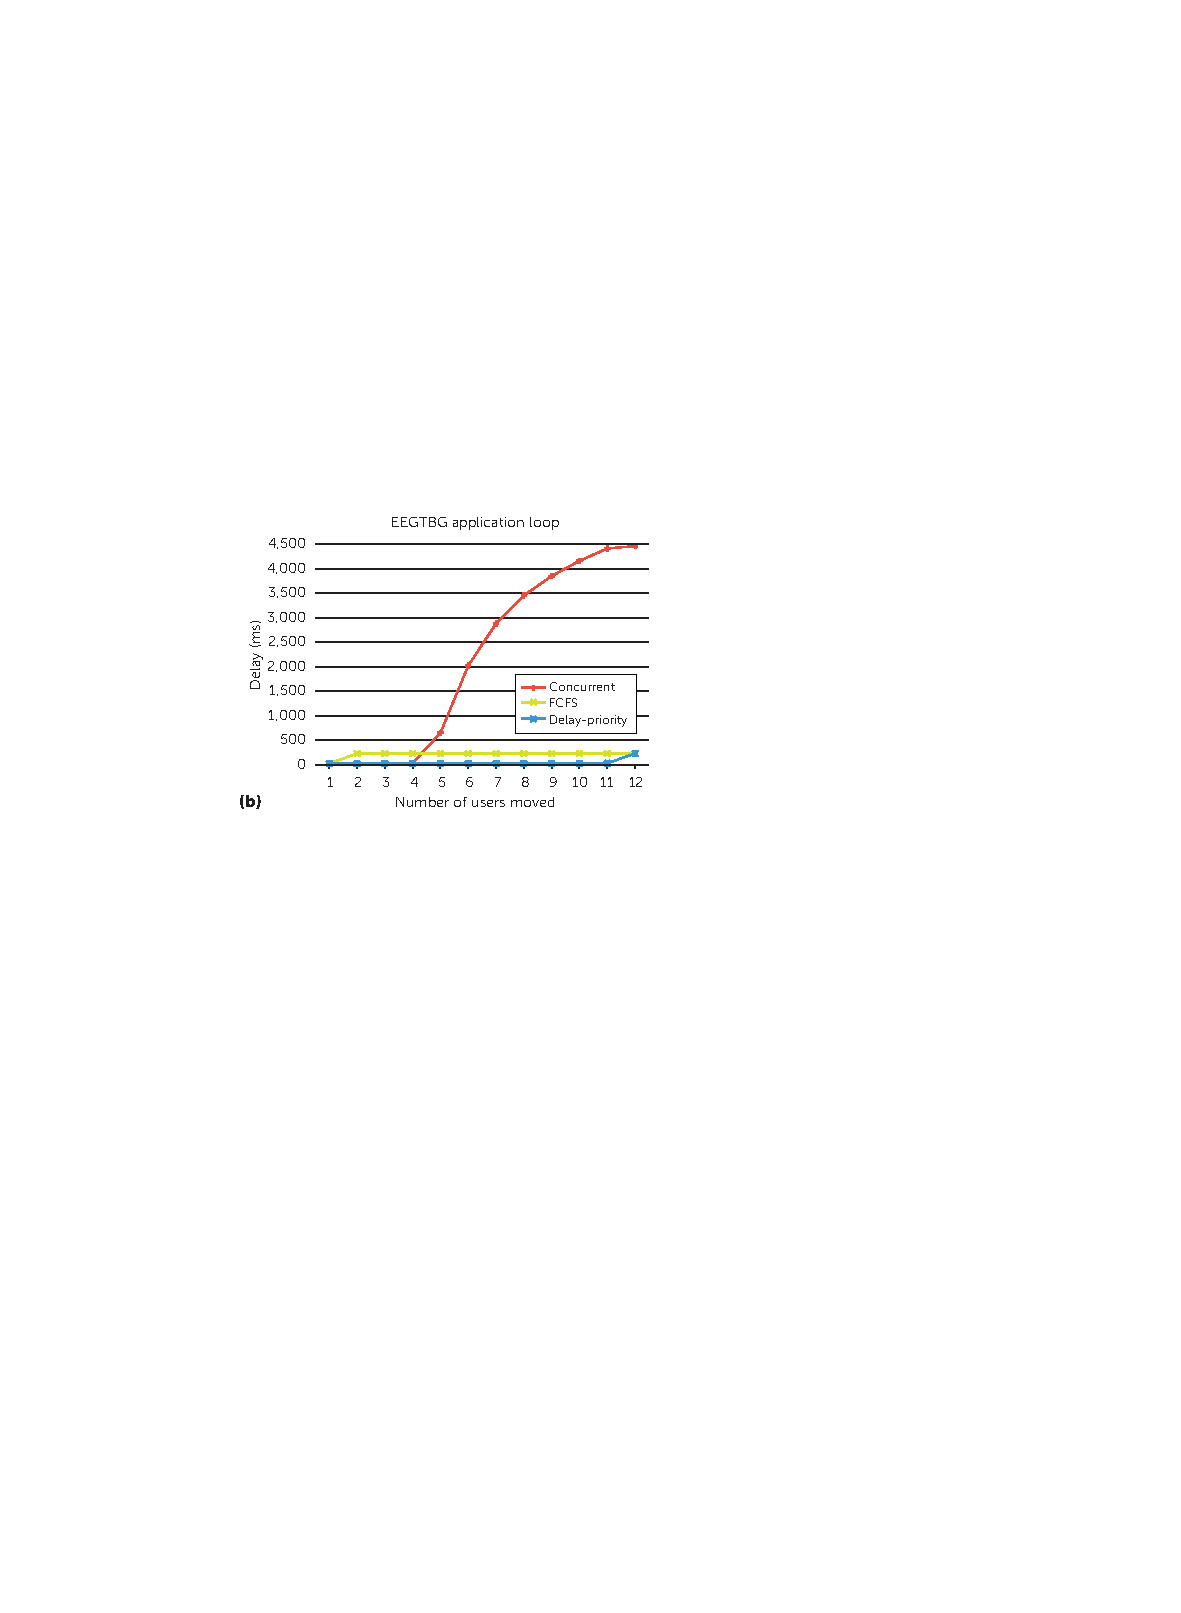
\includegraphics[scale=1.2]{images/4b.pdf}}
 		\caption[Application loop delays according to the scheduling strategy]{Application loop delays according to the scheduling strategy}
 	\end{figure}
\end{frame}

\begin{frame}
 	\begin{figure}[htbp]
 		\centerline{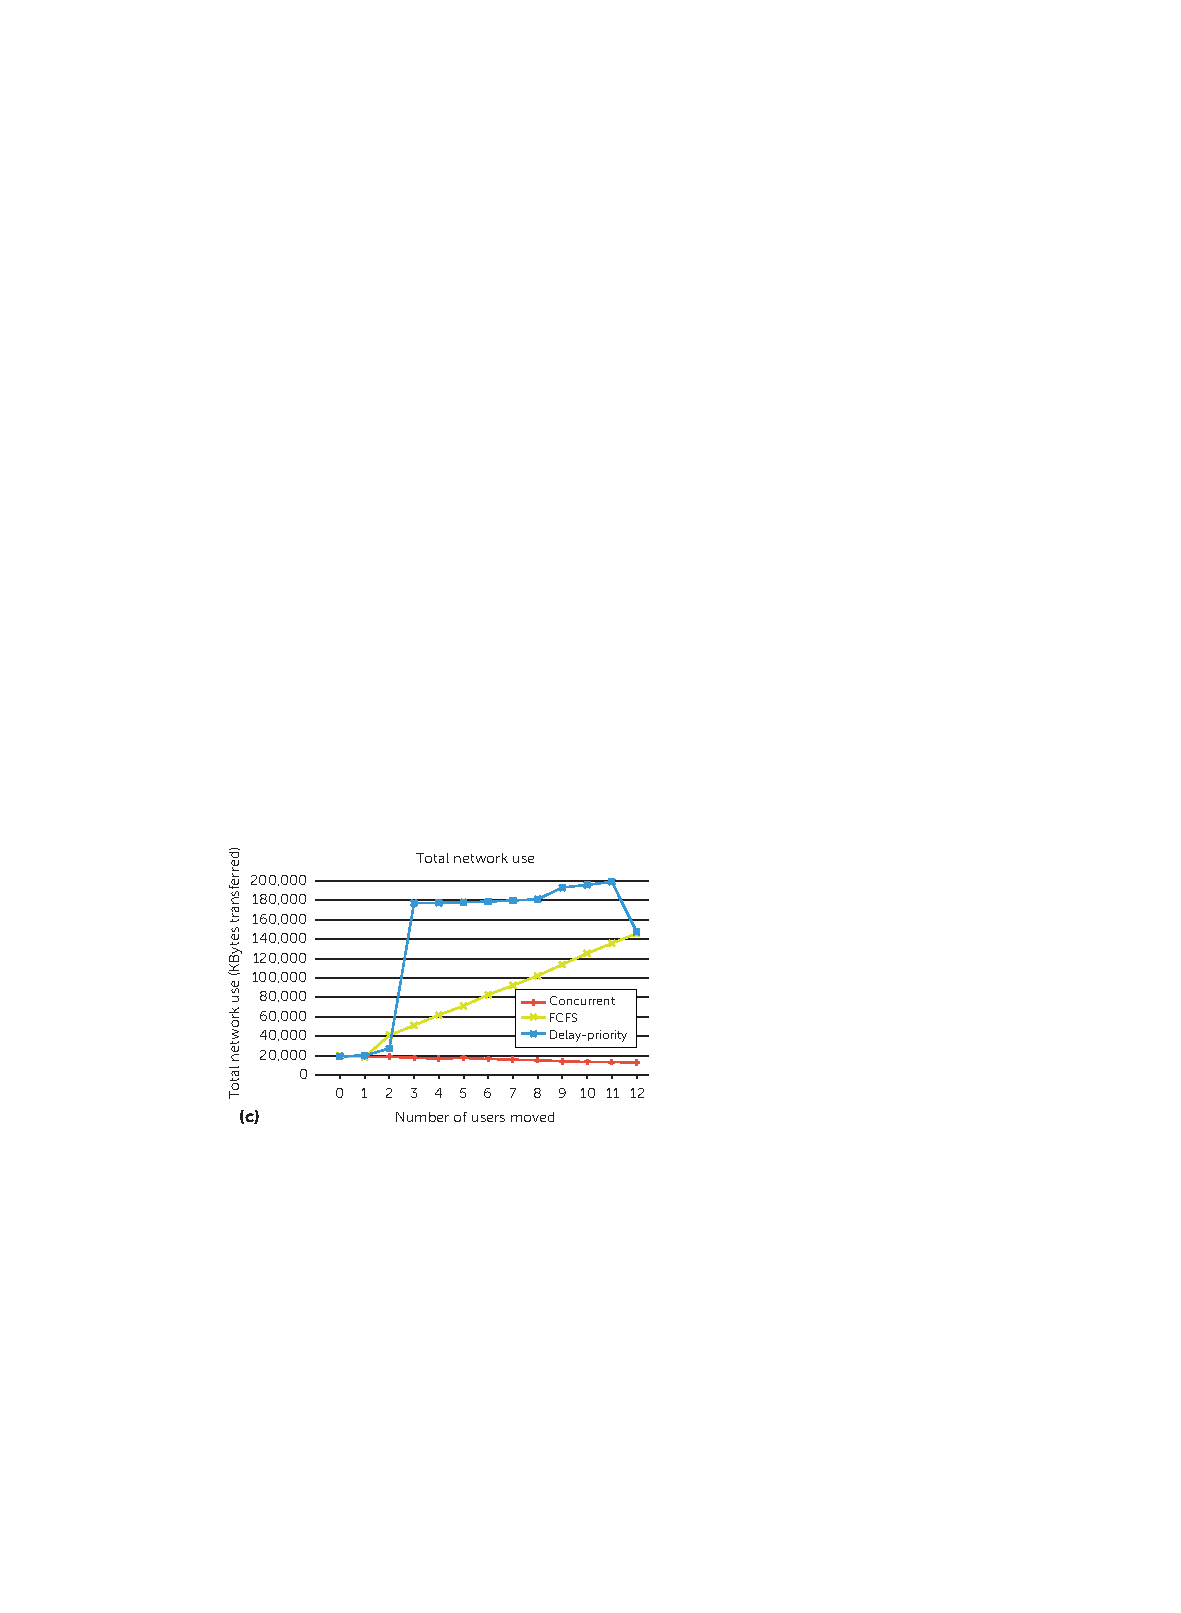
\includegraphics[scale=1.2]{images/4c.pdf}}
 		\caption[Network usage according to the scheduling strategy]{Network usage to the scheduling strategy}
 	\end{figure}
\end{frame}

\begin{frame}
 	\begin{figure}[htbp]
 		\centerline{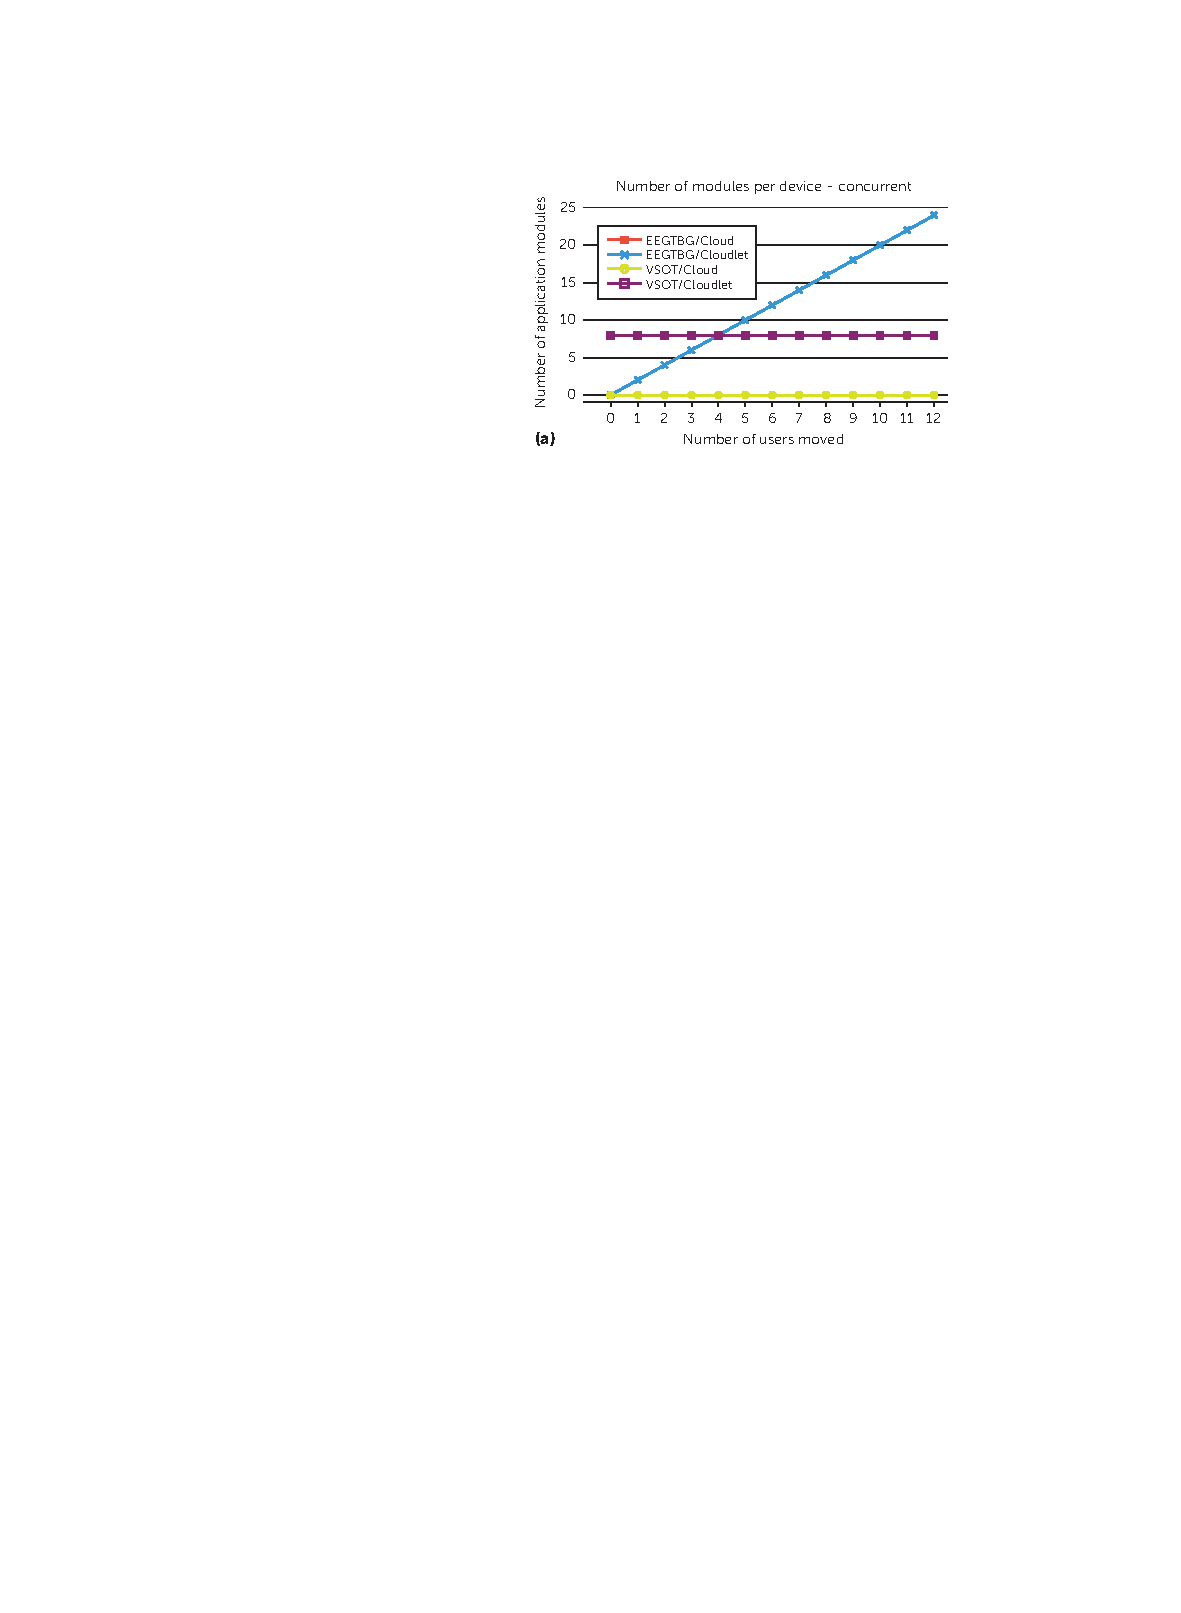
\includegraphics[scale=1.2]{images/5a.pdf}}
 		\caption[Number of modules per device - concurrent]{Number of modules per device - concurrent}
 	\end{figure}
\end{frame}

\begin{frame}
 	\begin{figure}[htbp]
 		\centerline{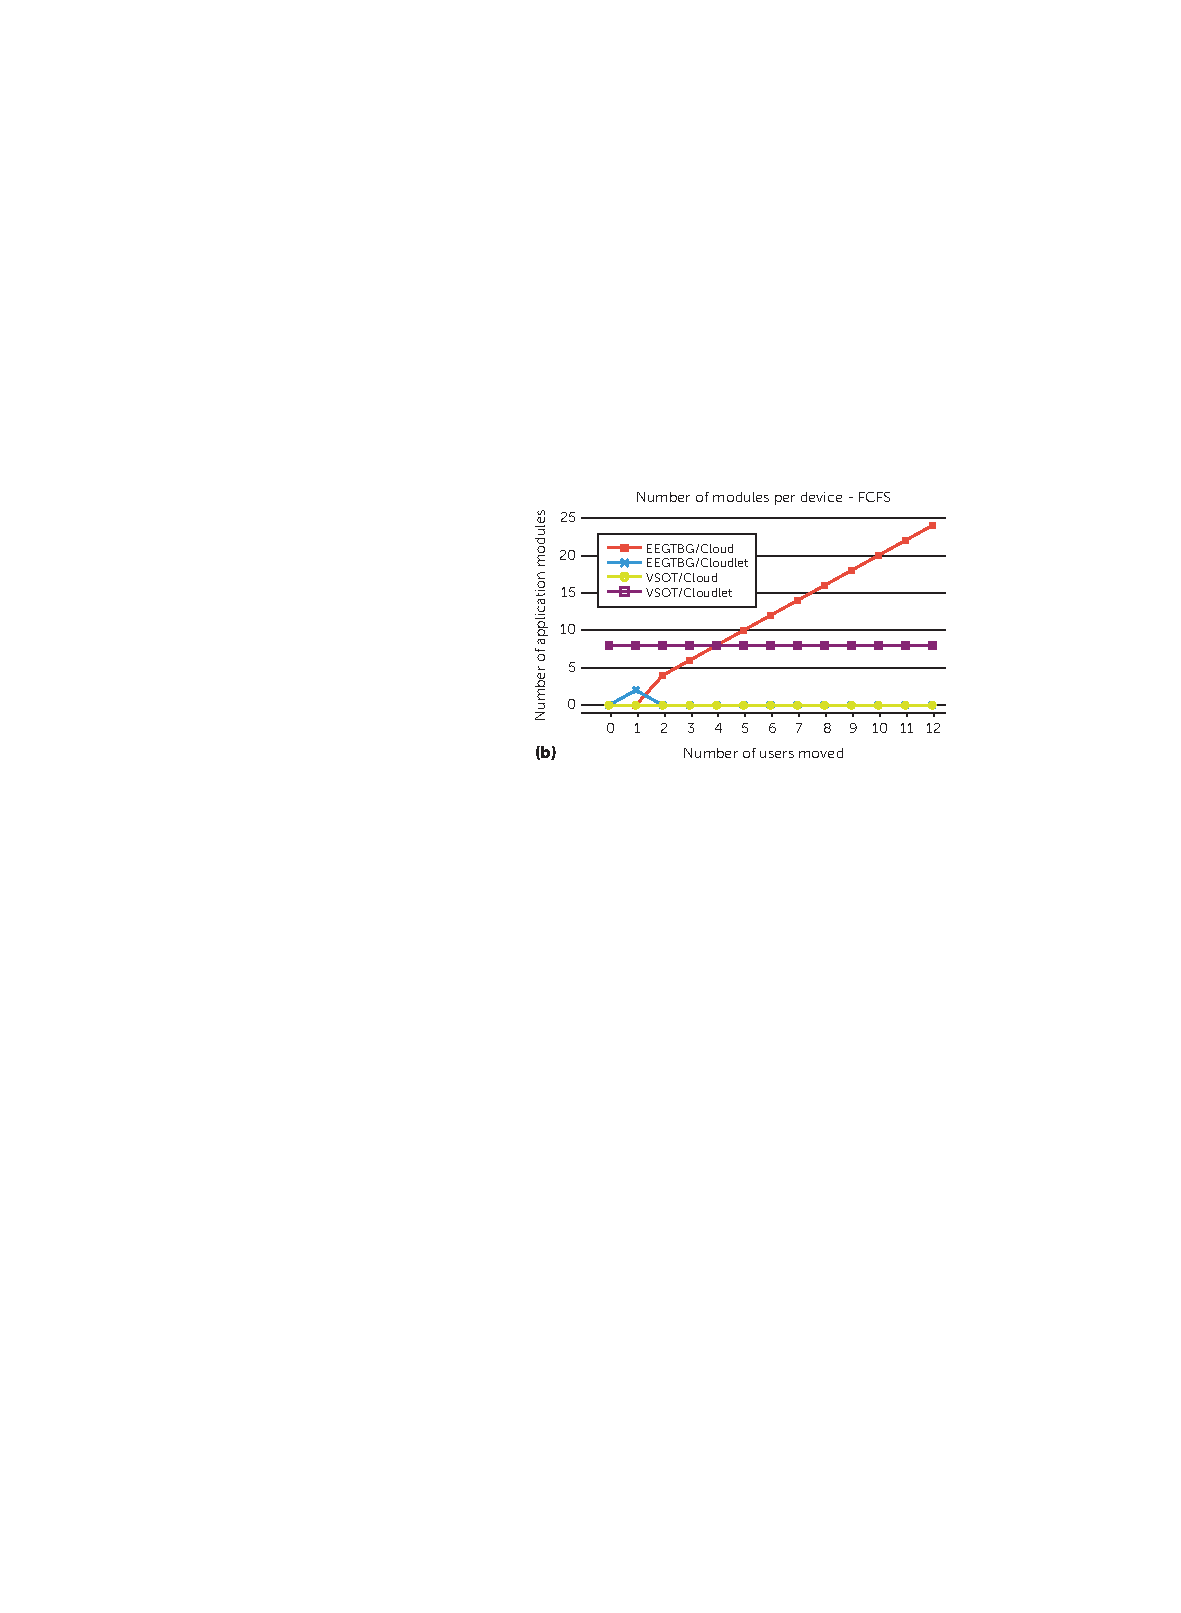
\includegraphics[scale=1.2]{images/5b.pdf}}
 		\caption[Number of modules per device - FCFS]{Number of modules per device - FCFS}
 	\end{figure}
\end{frame}

\begin{frame}
 	\begin{figure}[htbp]
 		\centerline{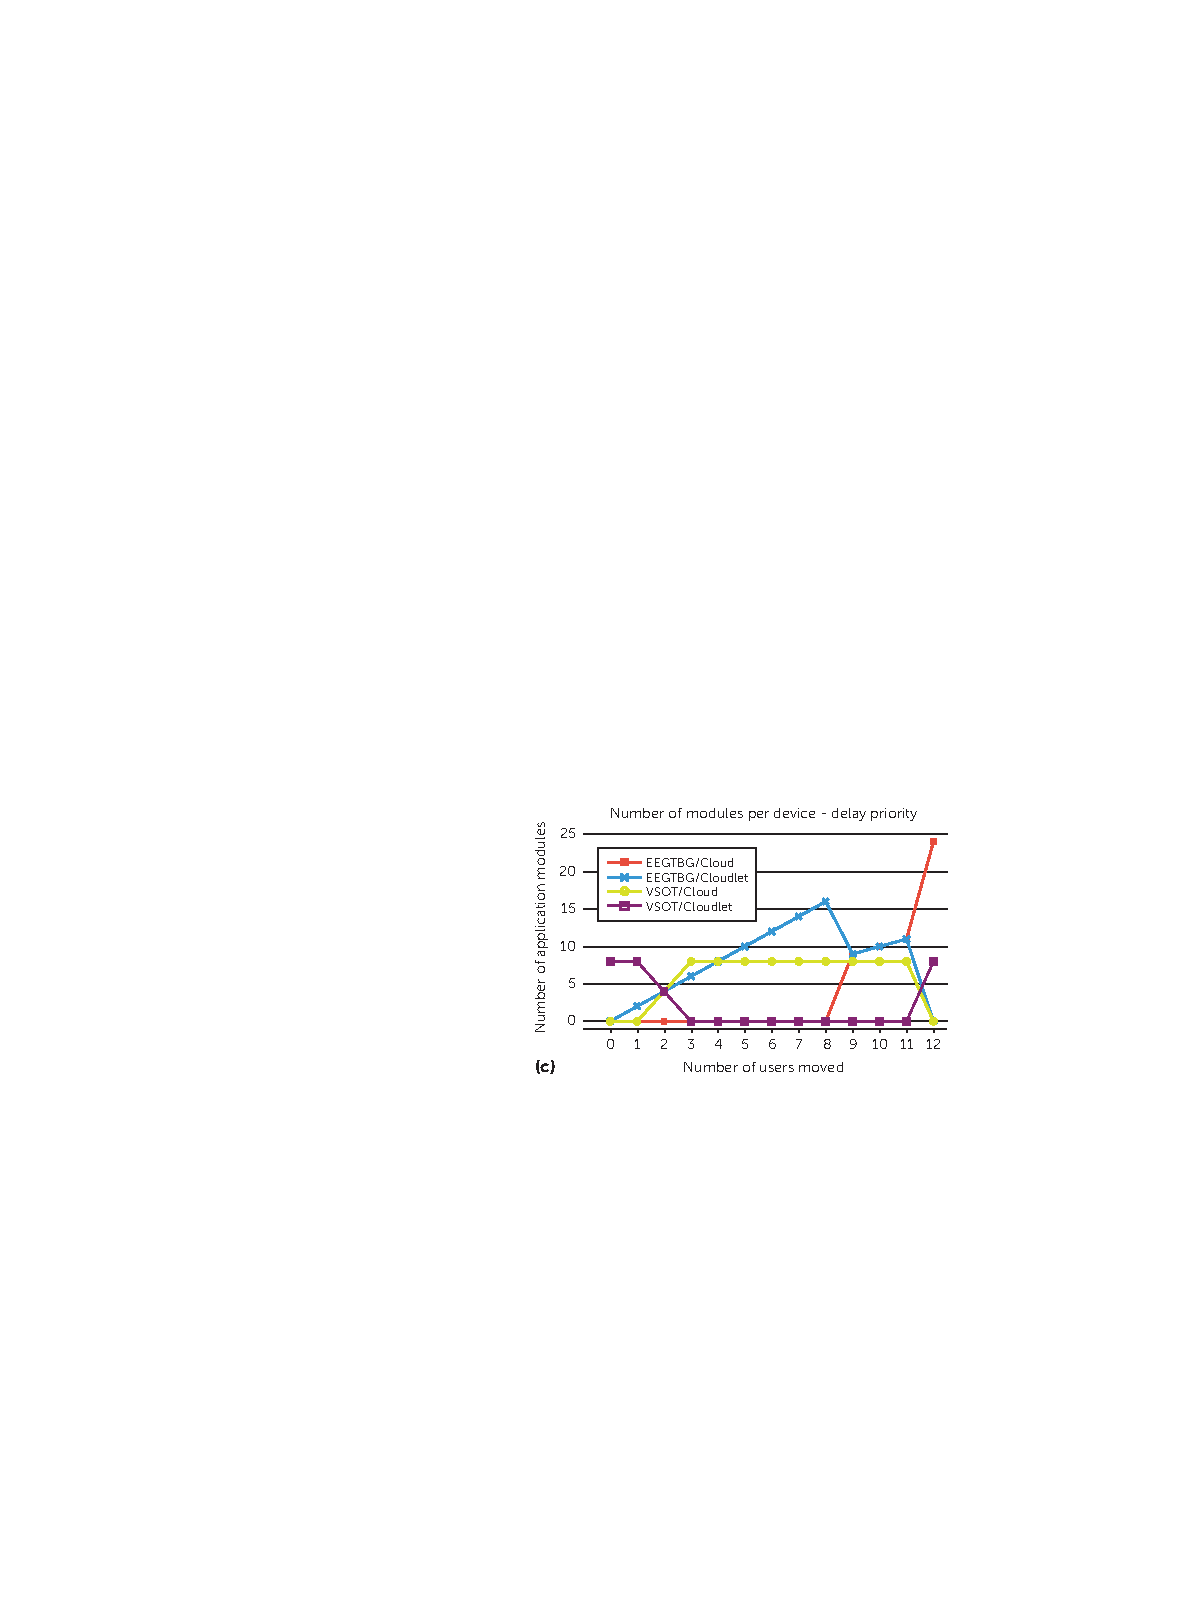
\includegraphics[scale=1.2]{images/5c.pdf}}
 		\caption[Number of modules per device - delay priority]{Number of modules per device - delay priority}
 	\end{figure}
\end{frame}

\section[Challenges and Future Directions]{Challenges and Future Directions}

\begin{frame}
	\tableofcontents[currentsection]
\end{frame}

\begin{frame}
	\frametitle{Challenges and Future Directions}
 	\begin{block}{}
 		\begin{itemize}
 			\item[•] \textbf{Application classification} and \textbf{user mobility} are key aspects to be associated with scheduling;\newline
 			\begin{itemize}
 				\item[-] \footnotesize\textit{The former, provide the scheduler with information about application requirements, which will allow the scheduler to prioritize the cloudlet use and other optimizations;}\newline
 		    	\item[-] \footnotesize\textit{The latter, improve resource management by better planning the applications scheduling beforehand. This planning is crucial to avoid application delays during user movement.}
 			\end{itemize}
 		\end{itemize}
 	\end{block}
\end{frame}

\begin{frame}
	\frametitle{Challenges and Future Directions}
 	\begin{block}{Some interesting areas to explore}
 		\begin{itemize}
 			\item[•] Strategies to deal with mobility prediction failure;\newline
 			\item[•] Maintaining connectivity without service disruption while migration occurs (resource virtualization, SDN);\newline
 			\item[•] Application execution costs in a fog utility model.
 		\end{itemize}
 	\end{block}
\end{frame}

\section[Conclusions]{Conclusions}

\begin{frame}
	\tableofcontents[currentsection]
\end{frame}

\begin{frame}
	\frametitle{Conclusions}
 	\begin{block}{}
 		\begin{itemize}
 			\item[•] Fog computing provides lower communication latencies and computing capacity closer to the final user;\newline
 			\item[•] For this infrastructure to become efficient, proper resource management mechanisms must be deployed;
 			\newline
 			\item[•] Scheduling strategies can be designed to cope with different application classes according to the demand coming from mobile users.
 		\end{itemize}
 	\end{block}
\end{frame}

% \begin{frame}{Dados do Artigo}
% \begin{minipage}{0.47\textwidth}
% 		\begin{itemize}
% 			\item[•] Accepted Date: 10/05/2017
% 			\item[•] Online Date: 13/06/2018
% 			\item[•] FI 2017: 1.105 (\textit{journal})
% 		\end{itemize}
% \end{minipage}
% \begin{minipage}{0.5\textwidth}
%     \begin{figure}[htbp]
% 		\centerline{
\includegraphics[scale=0.15]{images/fcs.jpg}}
% 			\label{fig:consolidatarefas6}
% 		\end{figure}
% \end{minipage}
% Acesso: \url{http://journal.hep.com.cn/fcs/EN/10.1007/s11704-017-6124-7}
% \end{frame}

%\section{Referências}
%
%\begin{frame}
%	\tableofcontents[currentsection]
%\end{frame}
%
%\begin{frame}[allowframebreaks]
%	\frametitle{Referências}
%	\def\newblock{}
%	\bibliographystyle{plain}
%	\tiny \bibliography{bibliografia}
%\end{frame}

% \section*{Agradecimentos}
	
% \begin{frame}
% 	\begin{center}
% 		\textbf{Obrigado!}
% 	\end{center}
% 	\begin{figure}[htbp]
% 		\begin{center}
% 			
\includegraphics[scale=.09]{images/Question-Mark.jpg}
% 		\end{center}
% 	\end{figure}
% 	\begin{center}
% 		\url{madsantos@inf.ufpel.edu.br}
% 	\end{center}
% \end{frame}

%%%%%%%%%%%%%%%%%%%%%%%%%%%%%%%%%%%%%%%%%%%%
% Último Slide
%%%%%%%%%%%%%%%%%%%%%%%%%%%%%%%%%%%%%%%%%%%%
\frame
{
	\pgfdeclareimage[height=1.5cm]{logo}{images/lups_oficial.png}
	\logo{\pgfuseimage{logo}
}	
	\logo{\vspace{3mm} 
	\begin{large}
		\textbf{Obrigado!} 
	\end{large}}
	\titlepage
}

\end{document}
